\documentclass[11pt,a4paper]{article}

\usepackage[T1]{fontenc}
\usepackage[utf8]{inputenc}
\usepackage{lmodern}
\usepackage{microtype}
\usepackage[a4paper,margin=1in]{geometry}
\usepackage{graphicx}
\usepackage{booktabs}
\usepackage{tabularx}
\usepackage{array}
\usepackage{amsmath}
\usepackage{adjustbox}
\usepackage{ragged2e}
\usepackage{caption}
\usepackage{hyperref}
\usepackage{xcolor}
\usepackage{tikz}
\usepackage{threeparttable}
\usepackage[section]{placeins}

\usetikzlibrary{arrows.meta,positioning,shapes.geometric}

\hypersetup{
  colorlinks=true,
  linkcolor=blue,
  urlcolor=blue,
  pdftitle={Quantum Vision Transformers Scientific Analysis Report},
  pdfauthor={Codex / reproduced\_papers workspace}
}

\pdfstringdefDisableCommands{%
  \def\repo{quantum_vision_transformers}%
  \def\papertitle{Quantum Vision Transformers}%
  \def\texttt#1{#1}%
  \def\_{}%
}

\setlength{\parskip}{0.55em}
\setlength{\parindent}{0pt}
\setlength{\emergencystretch}{2em}
\setlength{\tabcolsep}{5pt}
\renewcommand{\arraystretch}{1.18}
\captionsetup{font=small,labelfont=bf}

\newcommand{\repo}{\texttt{quantum\_vision\_transformers}}
\newcommand{\papertitle}{\textit{Quantum Vision Transformers}}
\newcolumntype{Y}{>{\RaggedRight\arraybackslash}X}
\newcolumntype{L}[1]{>{\RaggedRight\arraybackslash}p{#1}}

\title{\papertitle:\\Scientific Analysis, Reproduction Audit, and Extension Study}
\author{Prepared in the \texttt{reproduced\_papers} workspace}
\date{April 20, 2026}

\begin{document}
\maketitle

\begin{abstract}
This report presents a scientific audit of the current \repo{} repository with respect to the paper \papertitle{} (\texttt{2209.08167v2}). The project began as a direct reproduction effort and evolved into a broader experimental platform, but its central question remained stable: do the paper's quantum vision transformer ideas survive reimplementation, rerunning, and comparison against their stated classical and quantum baselines? The answer is positive at the qualitative level. The repository now supports a credible reproduction of the paper's main architectural findings, especially for models \texttt{A} and \texttt{D}, and it strongly supports the paper's parameter-efficiency argument. The reproduction is not, however, an exact numerical replica of every reported benchmark value. Model \texttt{B} is consistently weaker than the paper suggests, and the corrected paper-faithful \texttt{OrthoFNN} rerun remains materially below the paper baseline. Beyond reproduction, the repository now contains scientifically meaningful extension studies on lite operating points, capped-data MedMNIST training, and higher-order compound models. The strongest repository extension is \texttt{D\_full}; the clearest broader conclusion is that the compound family remains the most promising direction when training budgets are constrained.
\end{abstract}

\tableofcontents
\clearpage

\section{Introduction}

The paper \papertitle{} proposes several photonic alternatives to the attention mechanisms used in classical vision transformers. Its scientific appeal rests on two claims. First, structured quantum attention mechanisms can be trained and can perform competitively on MedMNIST-style image classification tasks. Second, these mechanisms are attractive because they use substantially fewer trainable attention parameters than a classical vision transformer baseline. The present repository was created to test those claims, initially through direct reimplementation and later through a larger set of comparative experiments and engineering corrections.

This document is written as a scientific report rather than as an experiment log. It explains how the repository models correspond to the paper models, what changes were required before the experiments became trustworthy, where the current evidence reproduces the paper, and where it diverges. It also documents the extension studies that emerged once the direct benchmark path was stable enough to support broader analysis.

One completion caveat should be stated at the outset. The MedMNIST butterfly-lite \texttt{train\_subset\_5000} sweep is complete for all \texttt{A}, \texttt{B}, and \texttt{D\_full} runs, but three plain-\texttt{D} seeds remain unfinished: one OCTMNIST seed and two TissueMNIST seeds. By contrast, the paper-faithful \texttt{OrthoFNN} rerun is now complete: the dedicated no-residual baseline path and grayscale image-wide embedding are both in place, so the remaining \texttt{OrthoFNN} gap should be treated as a genuine reproduction discrepancy rather than as a known implementation omission.

\section{Benchmark Scope and Model Families}

\subsection{Direct paper benchmark family}

The paper's simulation benchmark is narrower than the full repository model family. The direct paper-facing benchmark consists of five architectures: \texttt{VisionTransformer}, \texttt{OrthoFNN}, \texttt{A}, \texttt{B}, and \texttt{D}. In the repository, these correspond to the RetinaMNIST full-profile butterfly experiments and to the paper-style benchmark scripts using 100 epochs, batch size 32, Adam, learning rate \(10^{-3}\), and the learning-rate drops at epochs 50 and 75.

Table~\ref{tab:benchmark-family} summarizes the benchmark family in the narrower sense relevant for direct reproduction.

\begin{table}[tbp]
\centering
\caption{Paper benchmark family implemented in the repository.}
\label{tab:benchmark-family}
\small
\begin{tabularx}{\textwidth}{L{3.1cm}L{1.5cm}L{4.0cm}Y}
\toprule
Model & Photons & Primary mechanism & Role in the benchmark \\
\midrule
VisionTransformer & classical & Standard learned token-token attention with softmax & Classical reference baseline. \\
OrthoFNN & 1 & Repeated orthogonal feature transforms with no explicit attention & Quantum baseline without attention. \\
A & 1 & Shared one-photon orthogonal transform on token features & Paper core model testing whether orthogonal quantum mixing alone is competitive. \\
B & 1 & One-photon feature map \(V\) plus overlap-based quantum attention via \(W\) & Paper core transformer-like quantum attention model. \\
D & 2 & Two-photon compound interference with cross-sector readout & Paper core compound-attention model and the most natively quantum paper architecture. \\
\bottomrule
\end{tabularx}
\normalsize
\end{table}

\subsection{Repository extensions and exploratory variants}

The repository now contains models and operating regimes that were not part of the direct paper benchmark. They matter scientifically, but they should not be folded into a reproduction claim without qualification. Table~\ref{tab:extension-family} summarizes those additional models.

\begin{table}[tbp]
\centering
\caption{Repository extensions and exploratory variants.}
\label{tab:extension-family}
\small
\begin{tabularx}{\textwidth}{L{2.8cm}L{1.5cm}L{3.8cm}Y}
\toprule
Model & Photons & Primary mechanism & Scientific role in the repository \\
\midrule
C & 1 & Direct quantum attention using classically stored coefficients & Implemented for completeness and exploratory study, but not part of the paper's five-model simulation benchmark. \\
D\_full & 2 & Same compound layer as \texttt{D}, but with cross-, patch-, and feature-sector readout & Strongest repository extension so far; tests whether richer sector readout is beneficial. \\
E & 1+2 & Shared-circuit multi-sector attention & Exploratory tied-circuit hypothesis; interesting conceptually, but only weakly validated so far. \\
F & 3 & Hierarchical region-patch-feature compound interference & Most substantial higher-photon extension and the clearest route toward an \(n\)-photon compound family. \\
\bottomrule
\end{tabularx}
\normalsize
\end{table}

\begin{figure}[tbp]
\centering
\begin{adjustbox}{max width=0.88\textwidth}
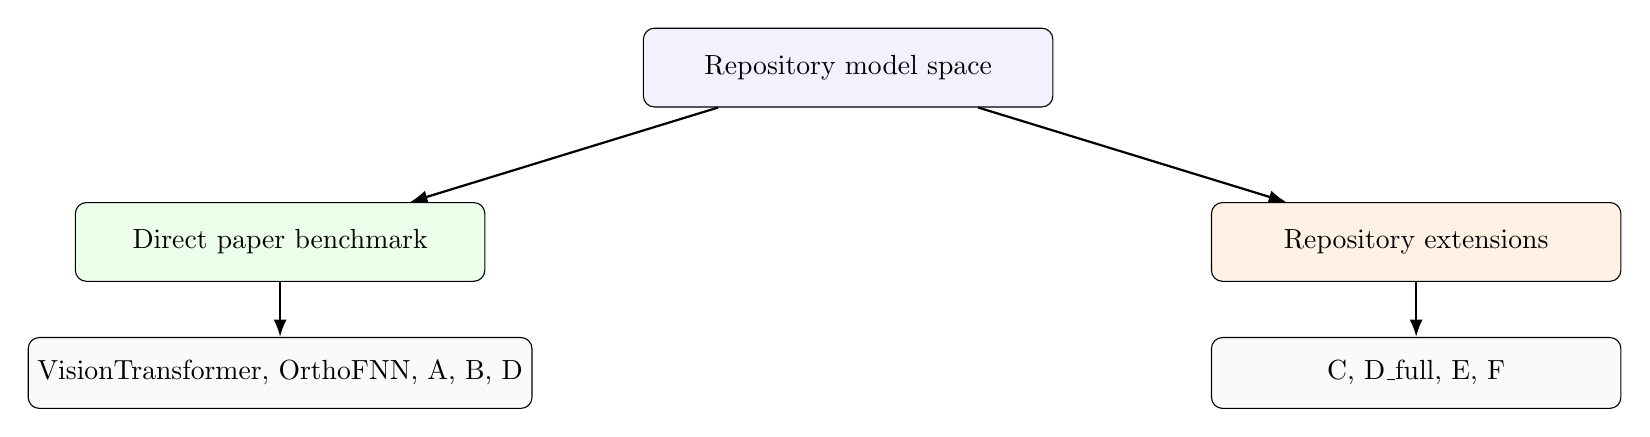
\begin{tikzpicture}[
  node distance=8mm,
  group/.style={draw, rounded corners, minimum width=52mm, minimum height=10mm, align=center, fill=blue!5},
  member/.style={draw, rounded corners, minimum width=52mm, minimum height=9mm, align=center, fill=gray!4},
  arrow/.style={-{Latex[length=2.2mm]}, thick}
]
\node[group] (root) {Repository model space};
\node[group, below left=12mm and 20mm of root, fill=green!8] (paper) {Direct paper benchmark};
\node[group, below right=12mm and 20mm of root, fill=orange!10] (ext) {Repository extensions};
\node[member, below=7mm of paper] (paperm) {VisionTransformer, OrthoFNN, A, B, D};
\node[member, below=7mm of ext] (extm) {C, D\_full, E, F};

\draw[arrow] (root) -- (paper);
\draw[arrow] (root) -- (ext);
\draw[arrow] (paper) -- (paperm);
\draw[arrow] (ext) -- (extm);
\end{tikzpicture}
\end{adjustbox}
\caption{Repository scope separated into the direct paper benchmark family and the extension family.}
\label{fig:model-scope}
\end{figure}

\subsection{Why model \texttt{C} is excluded from the direct reproduction claim}

Model \texttt{C} deserves explicit discussion because its presence in the repository can easily blur the distinction between reproduction and extension. The paper introduces Direct Quantum Attention in Section 3.3, but it does not use \texttt{C} as one of the five central architectures in the simulation benchmark. Instead, \texttt{C} is presented as an inference-oriented construction once attention coefficients have already been trained and stored classically. It is therefore a legitimate architecture from the paper, but not part of the exact benchmark family used to support the paper's main empirical claims. For that reason, \texttt{C} matters scientifically inside the repository, yet it is intentionally excluded from the narrow paper-facing reproduction statement.

\subsection{How the model families work}

The repository models differ not merely by parameter count or photon number, but by what ``attention'' means in each construction. Figure~\ref{fig:model-mechanics} condenses the major computational motifs into a more readable schematic than the raw code structure.

\begin{figure}[tbp]
\centering
\begin{adjustbox}{max width=\textwidth}
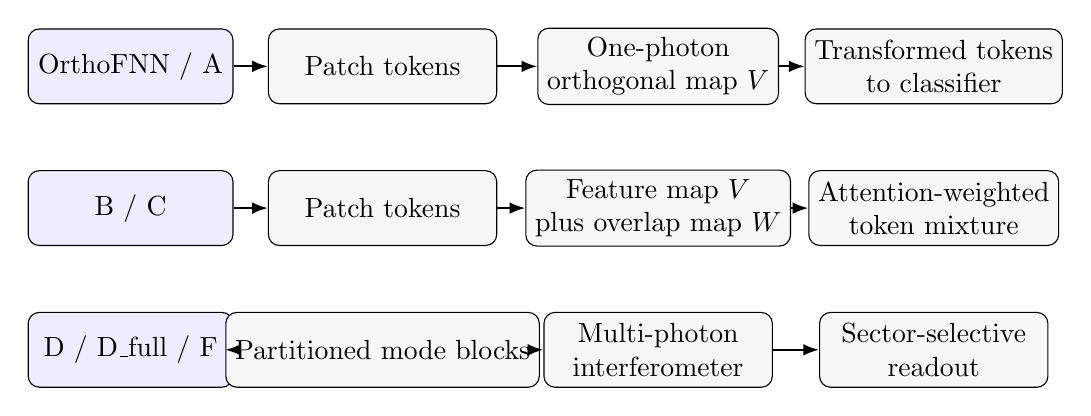
\begin{tikzpicture}[
  x=1cm, y=1cm,
  stage/.style={draw, rounded corners, minimum width=2.9cm, minimum height=0.95cm, align=center, fill=gray!6},
  fam/.style={draw, rounded corners, minimum width=2.6cm, minimum height=0.95cm, align=center, fill=blue!7},
  arrow/.style={-{Latex[length=2mm]}, thick}
]
\node[fam] (f1) at (1.8, 0) {OrthoFNN / A};
\node[stage] (f1a) at (5.0, 0) {Patch tokens};
\node[stage] (f1b) at (8.5, 0) {One-photon\\orthogonal map \(V\)};
\node[stage] (f1c) at (12.0, 0) {Transformed tokens\\to classifier};

\node[fam] (f2) at (1.8, -1.8) {B / C};
\node[stage] (f2a) at (5.0, -1.8) {Patch tokens};
\node[stage] (f2b) at (8.5, -1.8) {Feature map \(V\)\\plus overlap map \(W\)};
\node[stage] (f2c) at (12.0, -1.8) {Attention-weighted\\token mixture};

\node[fam] (f3) at (1.8, -3.6) {D / D\_full / F};
\node[stage] (f3a) at (5.0, -3.6) {Partitioned mode blocks};
\node[stage] (f3b) at (8.5, -3.6) {Multi-photon\\interferometer};
\node[stage] (f3c) at (12.0, -3.6) {Sector-selective\\readout};

\draw[arrow] (f1.east) -- (f1a.west);
\draw[arrow] (f1a.east) -- (f1b.west);
\draw[arrow] (f1b.east) -- (f1c.west);

\draw[arrow] (f2.east) -- (f2a.west);
\draw[arrow] (f2a.east) -- (f2b.west);
\draw[arrow] (f2b.east) -- (f2c.west);

\draw[arrow] (f3.east) -- (f3a.west);
\draw[arrow] (f3a.east) -- (f3b.west);
\draw[arrow] (f3b.east) -- (f3c.west);
\end{tikzpicture}
\end{adjustbox}
\caption{Representative computational motifs for the main model families. The figure distinguishes pure orthogonal feature mixing, explicit overlap-based attention, and compound multi-photon readout.}
\label{fig:model-mechanics}
\end{figure}

This distinction matters for interpretation. \texttt{OrthoFNN} and \texttt{A} test how far orthogonal feature mixing alone can go in the absence of explicit attention. \texttt{B} and \texttt{C} are closer in spirit to a classical transformer because they form a token-token weighting through overlap scores. \texttt{D}, \texttt{D\_full}, and \texttt{F} are more natively photonic: the attention effect is encoded implicitly by compound interference and readout sectors rather than by an explicit learned score matrix.

\subsection{Model-level schematics}

Because the paper mixes classical baselines, one-photon attention models, and multi-photon compound models, tables alone do not communicate the architectural differences well. The diagrams below summarize how the main models operate at the block level as implemented in the repository.

\begin{figure}[tbp]
\centering
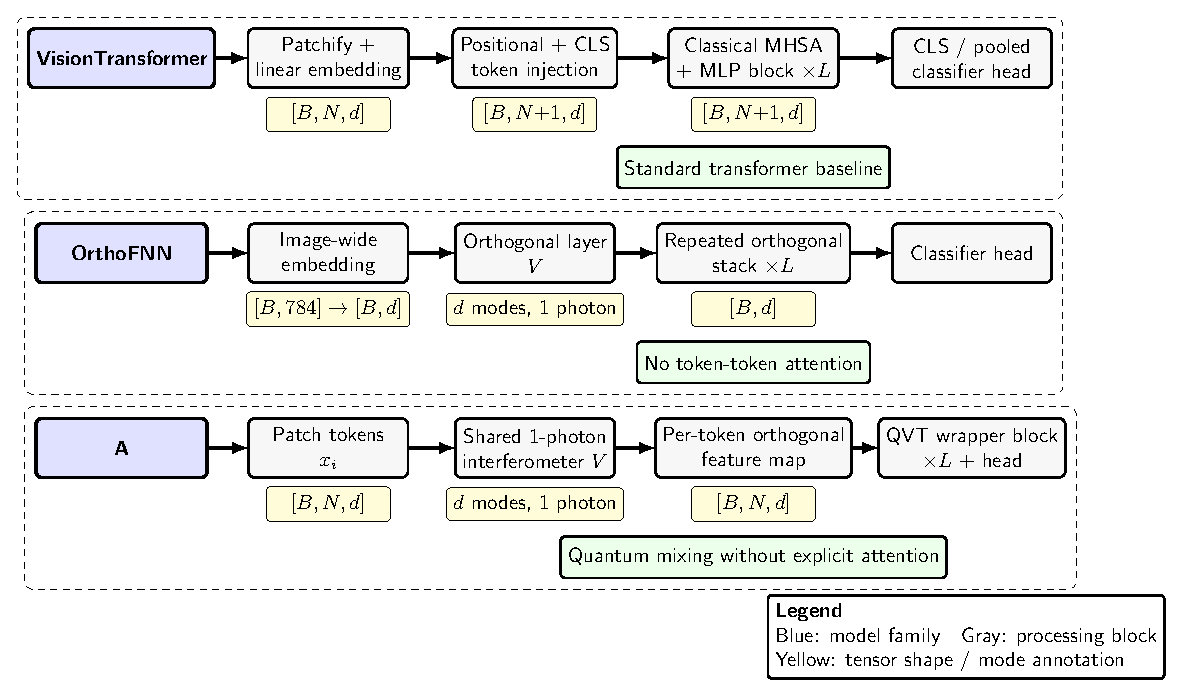
\includegraphics[width=\textwidth]{figures/arch_baselines_a.pdf}
\caption{Block-level view of the classical baseline, the no-attention quantum baseline, and paper model \texttt{A}. Yellow annotation boxes indicate tensor shapes or optical mode counts, so that the architectural similarity between \texttt{OrthoFNN} and \texttt{A} can be distinguished from their different input parameterizations.}
\label{fig:schematic-baselines-a}
\end{figure}

\begin{figure}[tbp]
\centering
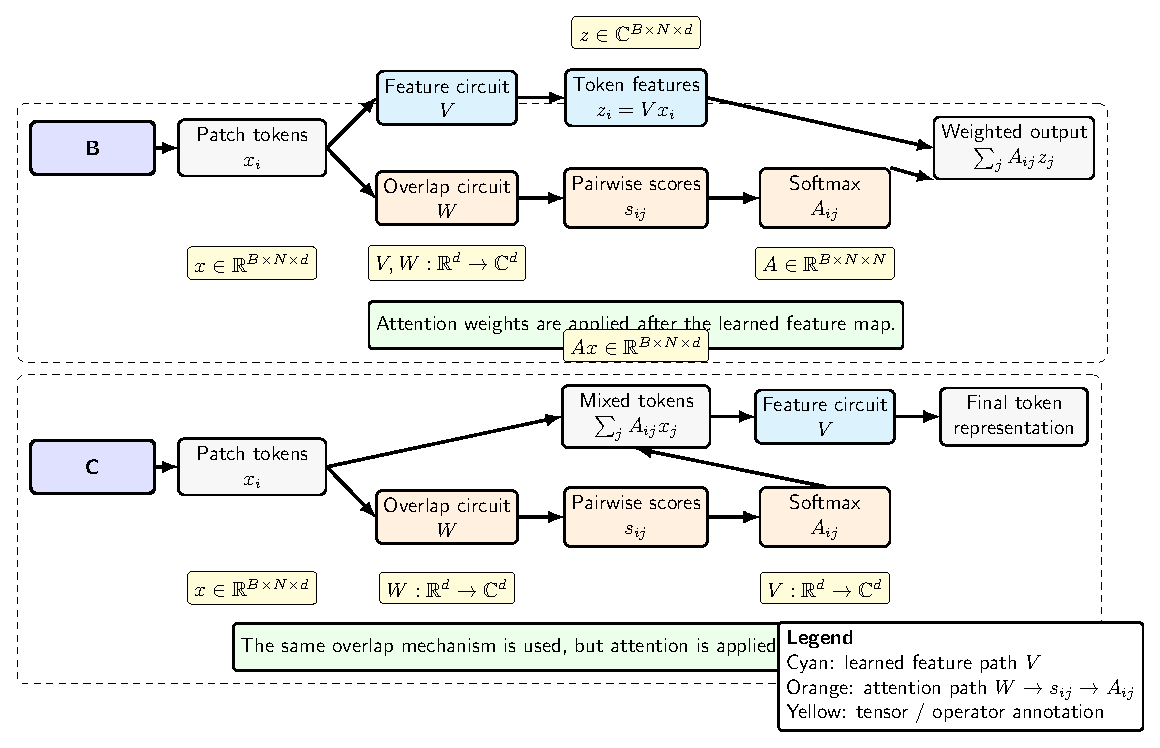
\includegraphics[width=\textwidth]{figures/arch_b_vs_c.pdf}
\caption{Schematic comparison of \texttt{B} and \texttt{C}. Cyan blocks denote the feature path, orange blocks denote the attention path, and yellow boxes record the tensor or operator types. In \texttt{B}, learned overlaps weight already transformed features. In \texttt{C}, the attention matrix is applied to the tokens first and only then passed through the final feature transform.}
\label{fig:schematic-bc}
\end{figure}

\begin{figure}[p]
\centering
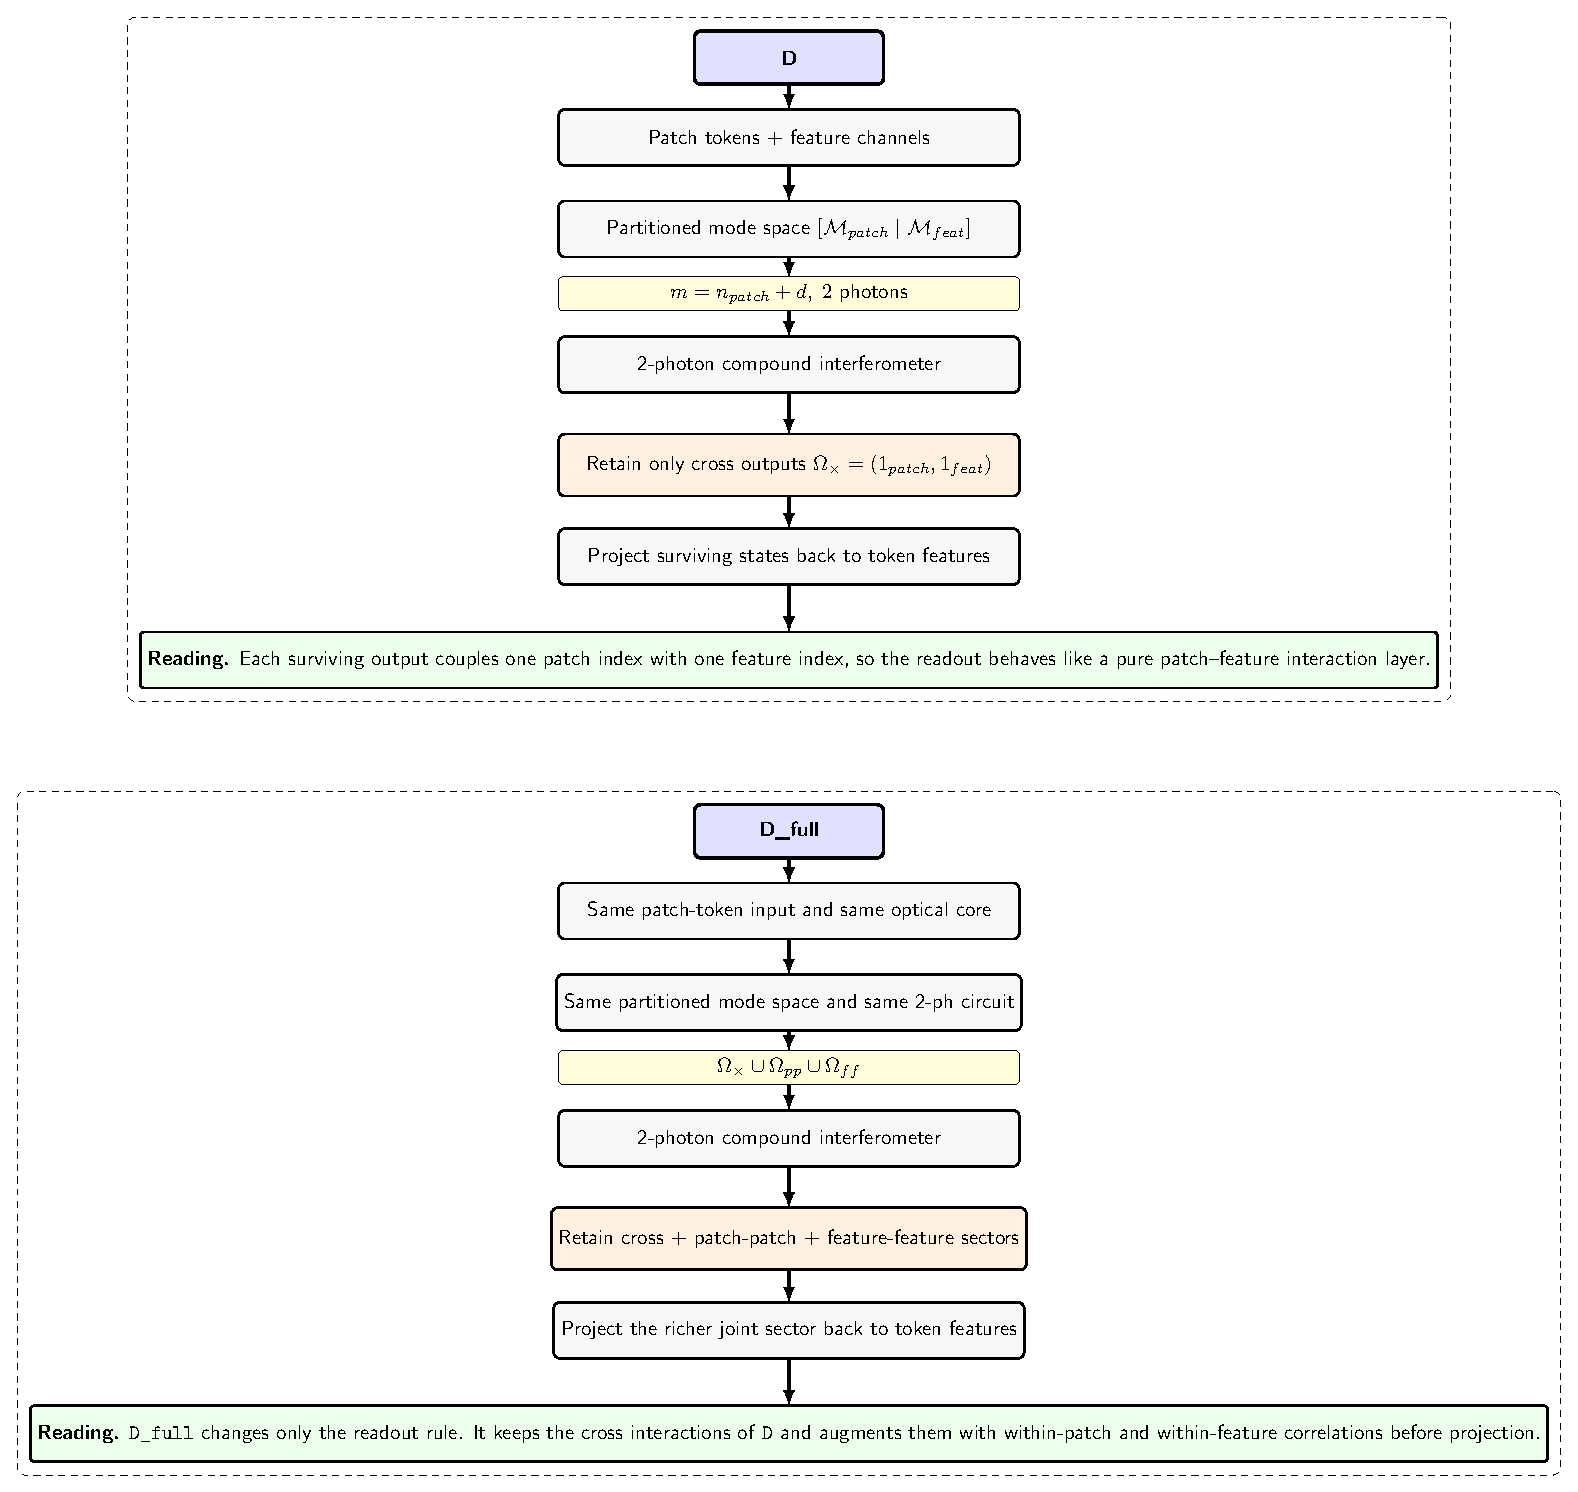
\includegraphics[width=\textwidth,height=0.86\textheight,keepaspectratio]{figures/arch_d_dfull.pdf}
\caption{Separated schematic for \texttt{D} and \texttt{D\_full}. The two models share the same compound optical core. The substantive difference is the retained output sector: \texttt{D} keeps only cross outputs, whereas \texttt{D\_full} also keeps same-block sectors before projection.}
\label{fig:schematic-ddfull}
\end{figure}

\begin{figure}[p]
\centering
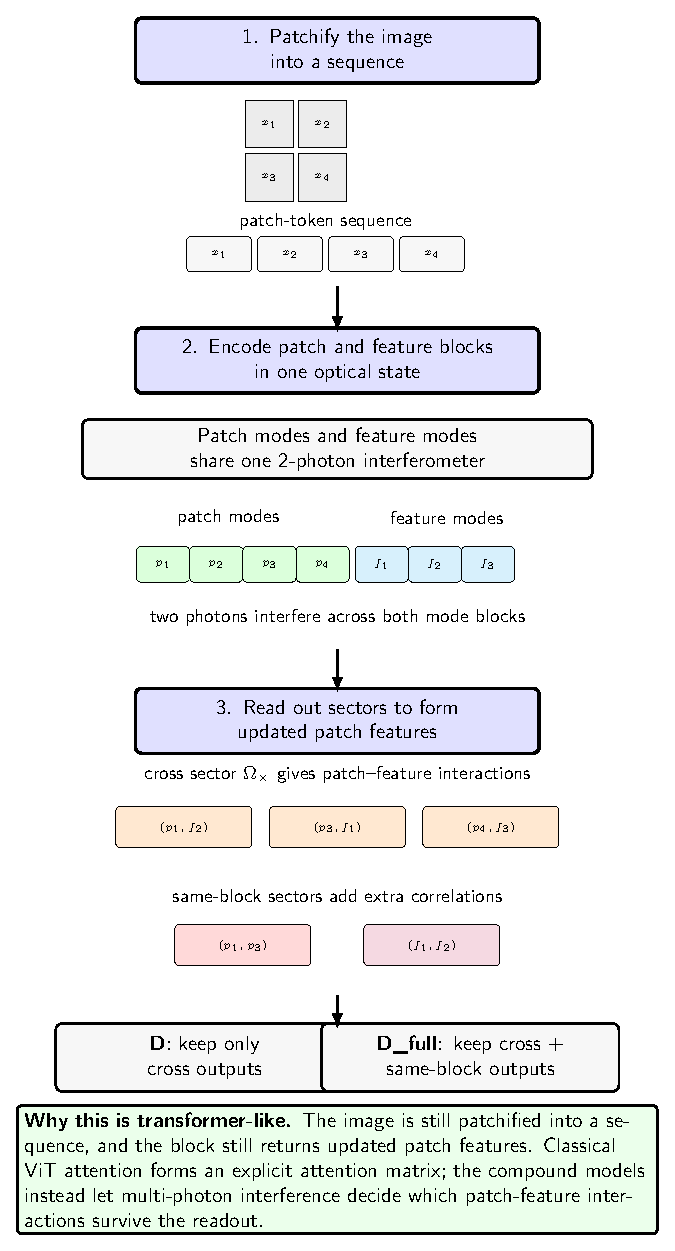
\includegraphics[width=\textwidth,height=0.86\textheight,keepaspectratio]{figures/compound_vision_intuition.pdf}
\caption{Image-level intuition for the compound transformer family. Image patches define one mode block, feature channels define another, and two-photon interference produces sector-specific outputs. The cross sector behaves like an attention-style patch-feature interaction; \texttt{D\_full} adds same-block correlations on top of that readout.}
\label{fig:compound-intuition}
\end{figure}

\begin{figure}[p]
\centering
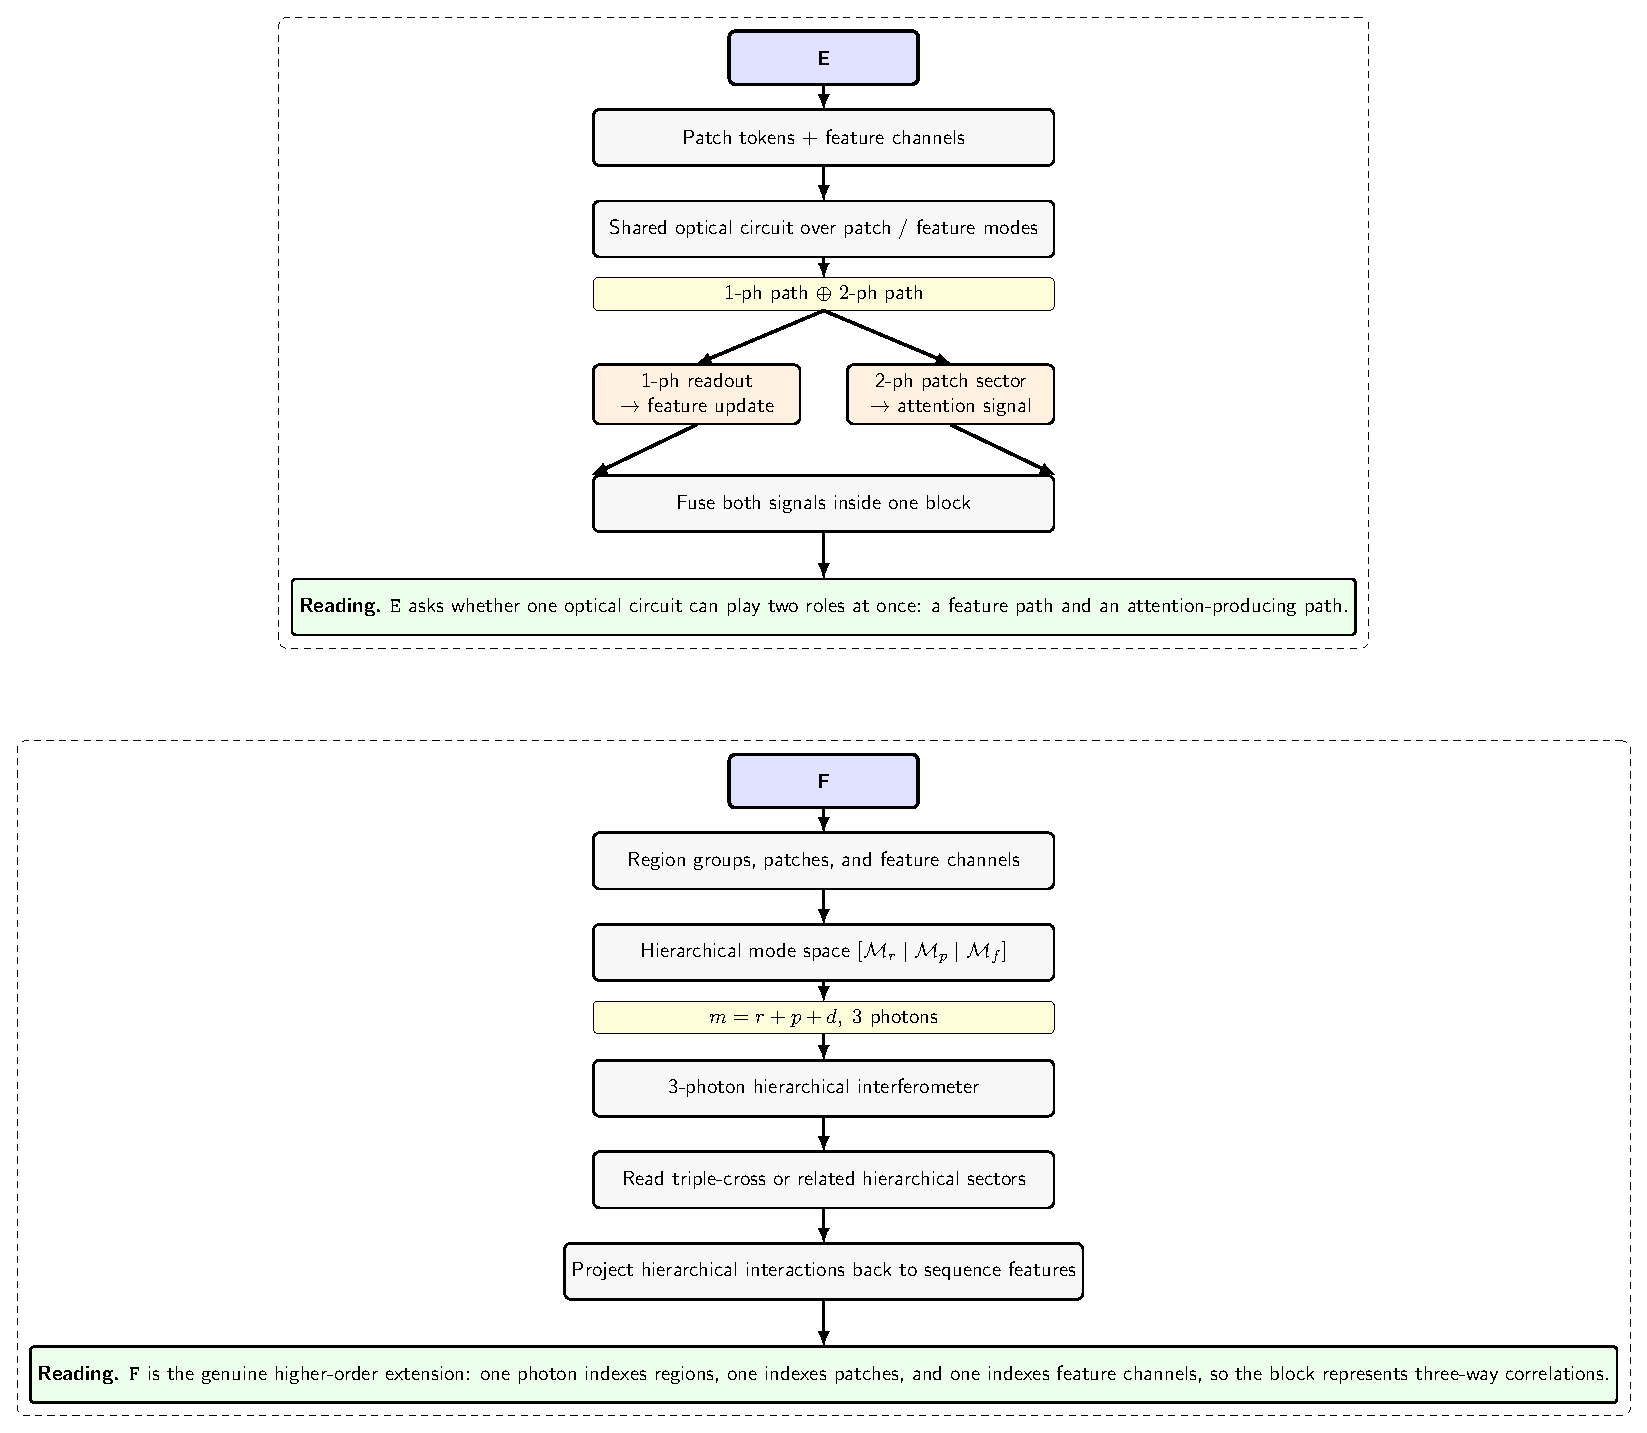
\includegraphics[width=\textwidth,height=0.84\textheight,keepaspectratio]{figures/arch_e_f.pdf}
\caption{Separated schematic for \texttt{E} and \texttt{F}. \texttt{E} shares one optical circuit across one- and two-photon readouts, while \texttt{F} is the genuine higher-order extension in which three photons encode a region--patch--feature hierarchy.}
\label{fig:schematic-ef}
\end{figure}

Figures~\ref{fig:schematic-baselines-a}--\ref{fig:schematic-ef} are useful for a practical reason as well. They show why some apparent modeling choices have different scientific status. The distinction between \texttt{B} and \texttt{C} is not cosmetic: it changes whether attention weights are applied before or after the learned quantum feature map. The distinction between \texttt{D} and \texttt{D\_full} lies almost entirely in the retained output sectors, whereas the distinction between \texttt{D} and \texttt{F} is a genuine increase in photon number and hierarchy.

Figure~\ref{fig:compound-intuition} is the more intuitive companion to the block diagrams. It visualizes why the compound models can still be thought of as vision-transformer-like architectures. The image is still split into patches, those patches still define a sequence-like structure, and the model still returns updated patch features. What changes is the mechanism: instead of explicitly forming an \(N\times N\) attention matrix, the compound block lets two photons interfere across patch and feature mode partitions, and then interprets the surviving sectors as structured patch-feature interactions.

\begin{figure}[tbp]
\centering
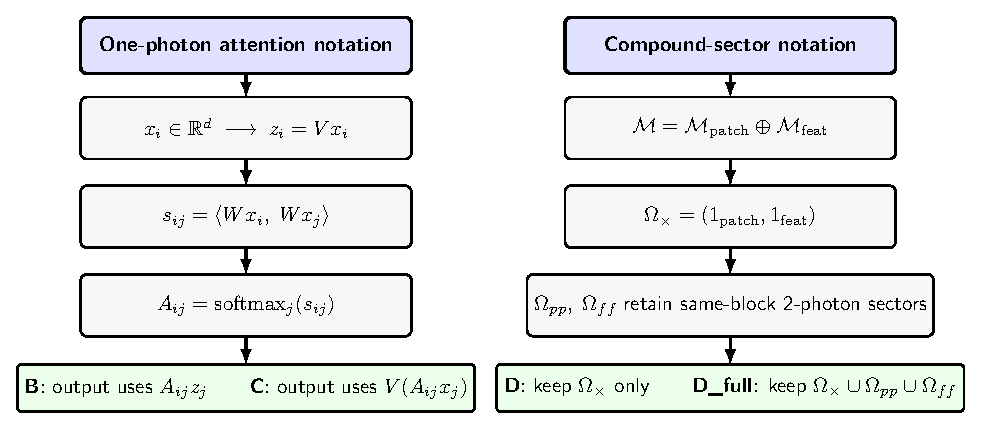
\includegraphics[width=\textwidth]{figures/notation_bridge.pdf}
\caption{Notation bridge between the repository diagrams and the paper's algebraic language. The left side summarizes the one-photon attention story in terms of \(V\), \(W\), score matrices, and softmax attention. The right side summarizes the partition and sector notation used by the compound-family models.}
\label{fig:notation-bridge}
\end{figure}

Figure~\ref{fig:notation-bridge} provides the direct bridge from the architectural plates to the paper's symbolic language. This is especially helpful because the repository models are implemented as executable modules rather than as equations. The notation bridge makes explicit that the one-photon family revolves around the operators \(V\) and \(W\), while the compound family revolves around partitioned mode spaces and sector selection such as \(\Omega_{\times}\), \(\Omega_{pp}\), and \(\Omega_{ff}\).

\section{Paper Counterparts and Implementation Fidelity}

The correctness of a reproduction claim depends not only on model names, but on whether the implementation matches the intended paper counterpart closely enough to justify comparison. Table~\ref{tab:counterparts} summarizes the current mapping between the paper-side models and the repository implementations.

\begin{table}[tbp]
\centering
\caption{Paper counterparts versus current repository implementations.}
\label{tab:counterparts}
\small
\begin{tabularx}{\textwidth}{L{3.0cm}Y Y}
\toprule
Model & Paper-side role & Current repository realization and caveat \\
\midrule
VisionTransformer & Classical baseline in the paper appendix and main benchmark tables & Direct classical baseline. On RetinaMNIST, the repository result already sits very close to the paper reference. \\
OrthoFNN & Quantum baseline without attention & Corrected to a dedicated no-residual, no-MLP path and rerun with the paper-faithful grayscale image-wide embedding. It still remains materially below the paper baseline. \\
A & Orthogonal Patch-wise Network & Direct paper model. Reproduction quality is strong in AUC, though ACC remains below the paper. \\
B & Orthogonal Transformer & Mechanistically faithful and directly benchmarked, but empirically weaker than the paper's headline impression. \\
C & Direct Quantum Attention & Implemented for exploration, but intentionally excluded from direct reproduction because the paper does not use it as one of the five benchmark models. \\
D & Compound Transformer & Direct paper model family. The repository butterfly path disables CLS to maintain a power-of-two mode count, which is the main architecture-level caveat. \\
D\_full, E, F & Repository extensions & Scientifically informative, but outside the paper's benchmark family. \\
\bottomrule
\end{tabularx}
\normalsize
\end{table}

\section{Methodology and Repository Corrections}

The repository did not begin in a state where scientific comparison to the paper was justified. Several engineering corrections were required before the results became interpretable. The most important changes were the repair of the structured butterfly circuits, safer checkpoint handling, deterministic data loading, broader automated tests, corrected paper benchmark scripts, more reliable figure generation, and substantial MerLin-side work to eliminate avoidable densification and to reroute the quantum layers through a more efficient execution path. These changes were aimed at preserving model semantics while removing implementation artifacts that would otherwise contaminate the scientific conclusions.

The direct paper-facing configuration in the repository is defined by RetinaMNIST, the \texttt{full} profile, the \texttt{butterfly} circuit family, and the five-model benchmark family \texttt{VisionTransformer}, \texttt{OrthoFNN}, \texttt{A}, \texttt{B}, and \texttt{D}. In that setting the repository closely matches the paper's stated training setup: 100 epochs, batch size 32, Adam, learning rate \(10^{-3}\), and learning-rate decay at epochs 50 and 75.

Three fidelity caveats remain important. First, the simulator stack is not identical to the paper's JAX-based implementation; the repository uses MerLin and Perceval-backed photonic simulation. Second, the butterfly implementation requires a power-of-two number of modes, which means that butterfly \texttt{D} disables the CLS token rather than constructing a 33-mode structured circuit. Third, the \texttt{OrthoFNN} baseline mismatch is now empirical rather than procedural: the paper-faithful rerun is complete, yet the baseline still trails the paper.

\section{RetinaMNIST: Direct Reproduction of the Paper Benchmark}

RetinaMNIST is the most defensible direct reproduction axis in the repository. It is explicitly emphasized in the paper, small enough to rerun reliably, and simple enough that deviations between paper and repository are easier to interpret than on the larger MedMNIST datasets.

\subsection{Paper-facing benchmark table}

Table~\ref{tab:retina-paper} compares the paper's RetinaMNIST values against the current regenerated butterfly/full means. The \texttt{OrthoFNN} row now reflects the completed paper-faithful rerun with the grayscale image-wide embedding.

\begin{table}[tbp]
\centering
\caption{RetinaMNIST butterfly/full benchmark comparison.}
\label{tab:retina-paper}
\small
\begin{tabularx}{\textwidth}{L{3.0cm}L{3.2cm}L{3.2cm}Y}
\toprule
Model & AUC (paper / repository) & ACC (paper / repository) & Interpretation \\
\midrule
VisionTransformer & 0.736 / 0.7417 $\pm$ 0.0030 & 0.548 / 0.5450 $\pm$ 0.0174 & Very close overall. The classical reference is reproduced well. \\
OrthoFNN & 0.731 / 0.6720 $\pm$ 0.0068 & 0.548 / 0.4908 $\pm$ 0.0059 & Clear mismatch even after the paper-faithful rerun. \\
A & 0.739 / 0.7479 $\pm$ 0.0071 & 0.560 / 0.5325 $\pm$ 0.0122 & Strong AUC match and credible qualitative reproduction. \\
B & 0.745 / 0.7369 $\pm$ 0.0053 & 0.542 / 0.5108 $\pm$ 0.0066 & Mechanistically faithful, but weaker than the paper suggests. \\
D & 0.740 / 0.7409 $\pm$ 0.0087 & 0.565 / 0.5283 $\pm$ 0.0077 & AUC matches closely; ACC remains consistently lower. \\
\bottomrule
\end{tabularx}
\normalsize
\end{table}

The result is mixed but scientifically meaningful. The repository reproduces the paper's qualitative story more convincingly than it reproduces every benchmark value exactly. \texttt{VisionTransformer}, \texttt{A}, and \texttt{D} are close enough to count as successful qualitative reproductions. \texttt{B} is weaker than expected, and the baseline side remains the least successful part of the comparison because \texttt{OrthoFNN} still underperforms the paper after the paper-faithful rerun.

\subsection{Figures and interpretation}

\begin{figure}[tbp]
\centering

\includegraphics[width=\textwidth]{../../figures/butterfly/full/comparison_retinamnist.png}
\caption{RetinaMNIST butterfly/full comparison for the paper benchmark family and the repository extension \texttt{D\_full}.}
\label{fig:retina-full-comparison}
\end{figure}

Figure~\ref{fig:retina-full-comparison} is the clearest paper-facing plot in the repository. It shows that \texttt{A} is the strongest quantum model by AUC in the direct butterfly/full setting, while \texttt{D} remains highly competitive and sits almost exactly on the paper's AUC level. The classical baseline is strong but not dominant. That behavior is precisely the qualitative story the paper aimed to establish. The main discrepancy is on the baseline side, where \texttt{OrthoFNN} is visibly weaker than the paper implies.

\begin{figure}[tbp]
\centering

\includegraphics[width=\textwidth]{../../figures/butterfly/full/training_curves_retinamnist.png}
\caption{RetinaMNIST butterfly/full training curves.}
\label{fig:retina-full-training}
\end{figure}

Figure~\ref{fig:retina-full-training} helps separate architectural mismatch from optimization failure. The stronger quantum models do not collapse during training; their curves are stable and interpretable. The remaining gap between repository and paper is therefore unlikely to be explained by simple optimization failure. It is more plausibly due to architecture-level details, simulator-stack differences, and output-calibration effects.

\begin{figure}[tbp]
\centering

\includegraphics[width=0.82\textwidth]{../../figures/butterfly/full/param_comparison.png}
\caption{RetinaMNIST parameter comparison.}
\label{fig:retina-param}
\end{figure}

Figure~\ref{fig:retina-param} is one of the strongest points of agreement between paper and repository. The quantum attention mechanisms use substantially fewer trainable attention parameters than the classical transformer baseline. Even where the benchmark numbers are not exact matches, the paper's parameter-efficiency claim is strongly supported by the regenerated results.

The scientifically careful conclusion from the direct RetinaMNIST benchmark is therefore clear. The repository reproduces the paper's central qualitative finding that structured quantum models can compete with the classical transformer baseline, especially through \texttt{A} and \texttt{D}. What it does not yet deliver is a clean model-by-model numerical replica across the entire benchmark family.

\section{Lite Operating Points on RetinaMNIST}

The lite profile began as an engineering convenience, but it turned into a scientifically interesting regime in its own right. Lite does not correspond to a shallower interferometer in the optical sense. Instead, it reduces outer model depth, feature width, and total trainable parameter count while keeping the model family itself intact. It is therefore best interpreted as a reduced-capacity operating point rather than as a different architecture.

\begin{table}[tbp]
\centering
\caption{RetinaMNIST butterfly lite versus full for overlapping models.}
\label{tab:lite-vs-full}
\small
\begin{tabularx}{\textwidth}{L{2.3cm}L{3.1cm}L{3.1cm}Y}
\toprule
Model & AUC (full / lite) & ACC (full / lite) & Interpretation \\
\midrule
A & 0.7479 / 0.7386 & 0.5325 / 0.5342 & Lite is very close to full despite the lower-capacity operating point. \\
B & 0.7369 / 0.7392 & 0.5108 / 0.5250 & Lite is modestly better, suggesting the full operating point may be unnecessarily large for RetinaMNIST. \\
D & 0.7409 / 0.7381 & 0.5283 / 0.5250 & Essentially tied. The compound mechanism survives the reduction well. \\
D\_full & 0.7313 / 0.7408 & 0.5225 / 0.5392 & Lite currently looks better, but the full comparison remains weak because the full side is sparsely sampled. \\
\bottomrule
\end{tabularx}
\normalsize
\end{table}

\begin{figure}[tbp]
\centering

\includegraphics[width=\textwidth]{../../figures/butterfly/lite/comparison_retinamnist.png}
\caption{RetinaMNIST butterfly-lite comparison.}
\label{fig:retina-lite-comparison}
\end{figure}

\begin{figure}[tbp]
\centering

\includegraphics[width=\textwidth]{../../figures/butterfly/lite/training_curves_retinamnist.png}
\caption{RetinaMNIST butterfly-lite training curves.}
\label{fig:retina-lite-training}
\end{figure}

The strongest inference from the lite study is not that lite is universally superior to full. Rather, lite often preserves most of the useful behavior of the full models. On RetinaMNIST, that suggests the paper-style operating point may be somewhat over-capacity for the dataset. This does not invalidate the paper. It instead indicates that the paper chose a reasonable benchmark point, but not necessarily the most data-efficient operating point for a small dataset of this scale.

\section{MedMNIST Under Capped Training Budgets}

The MedMNIST study extends the paper rather than reproduces it exactly. A full CPU sweep of the paper benchmark family across all datasets is expensive enough that it is poorly suited to rapid iteration, so the repository introduced capped-data regimes to study data efficiency while preserving the official validation and test splits.

The earliest capped-data regime, \texttt{retina\_sized\_train}, was most useful as a negative result. It showed that several large MedMNIST datasets are too data-hungry for a Retina-sized training ceiling. PathMNIST makes the point clearly: increasing the training budget from 1080 examples to 5000 examples substantially improves both AUC and ACC.

\begin{table}[tbp]
\centering
\caption{PathMNIST under Retina-sized versus 5k-capped training.}
\label{tab:pathmnist-cap}
\small
\begin{tabularx}{\textwidth}{L{2.0cm}Y Y}
\toprule
Model & Retina-sized training & 5k-capped training \\
\midrule
A & 0.8768 AUC / 0.5445 ACC & 0.9434 AUC / 0.6468 ACC \\
B & 0.8473 AUC / 0.4499 ACC (single completed seed) & 0.9300 AUC / 0.6681 ACC \\
\bottomrule
\end{tabularx}
\normalsize
\end{table}

The more informative MedMNIST result is the butterfly-lite \texttt{train\_subset\_5000} regime. All \texttt{A}, \texttt{B}, and \texttt{D\_full} runs are now complete; only three plain-\texttt{D} seeds remain outstanding. To avoid forcing the report into an unreadable single wide table, the results are split across two tables below.

\begin{table}[tbp]
\centering
\caption{Butterfly-lite \texttt{train\_subset\_5000} results, part I. Each entry is reported as AUC / ACC.}
\label{tab:subset5000-a}
\small
\begin{tabularx}{\textwidth}{L{2.8cm}L{2.3cm}L{2.3cm}L{2.3cm}Y}
\toprule
Dataset & A & B & D & D\_full \\
\midrule
bloodmnist & 0.9647 / 0.7899 & 0.9681 / 0.7985 & 0.9754 / 0.8351 & 0.9740 / 0.8243 \\
breastmnist & 0.7875 / 0.7756 & 0.8341 / 0.7821 & 0.8095 / 0.8013 & 0.8059 / 0.7714 \\
dermamnist & 0.8745 / 0.7099 & 0.8647 / 0.7016 & 0.8927 / 0.7272 & 0.8884 / 0.7177 \\
octmnist & 0.7700 / 0.4583 & 0.7692 / 0.4617 & 0.8177 / 0.5050 (n=2) & 0.8173 / 0.5070 \\
\bottomrule
\end{tabularx}
\normalsize
\end{table}

\begin{table}[tbp]
\centering
\caption{Butterfly-lite \texttt{train\_subset\_5000} results, part II. Each entry is reported as AUC / ACC.}
\label{tab:subset5000-b}
\small
\begin{tabularx}{\textwidth}{L{2.8cm}L{2.3cm}L{2.3cm}L{2.3cm}Y}
\toprule
Dataset & A & B & D & D\_full \\
\midrule
pathmnist & 0.9434 / 0.6468 & 0.9300 / 0.6681 & 0.9410 / 0.6742 & 0.9452 / 0.6762 \\
pneumoniamnist & 0.9439 / 0.8456 & 0.9428 / 0.8691 & 0.9507 / 0.8590 & 0.9473 / 0.8632 \\
retinamnist & 0.7387 / 0.5342 & 0.7390 / 0.5300 & 0.7381 / 0.5250 & 0.7408 / 0.5392 \\
tissuemnist & 0.8106 / 0.5017 & 0.8055 / 0.4917 & 0.8167 / 0.5123 (n=2) & 0.8209 / 0.5145 \\
\bottomrule
\end{tabularx}
\normalsize
\end{table}

\begin{figure}[tbp]
\centering

\includegraphics[width=\textwidth]{../../figures/butterfly/lite/comparison_pathmnist.png}
\caption{PathMNIST butterfly-lite comparison.}
\label{fig:pathmnist}
\end{figure}

\begin{figure}[tbp]
\centering
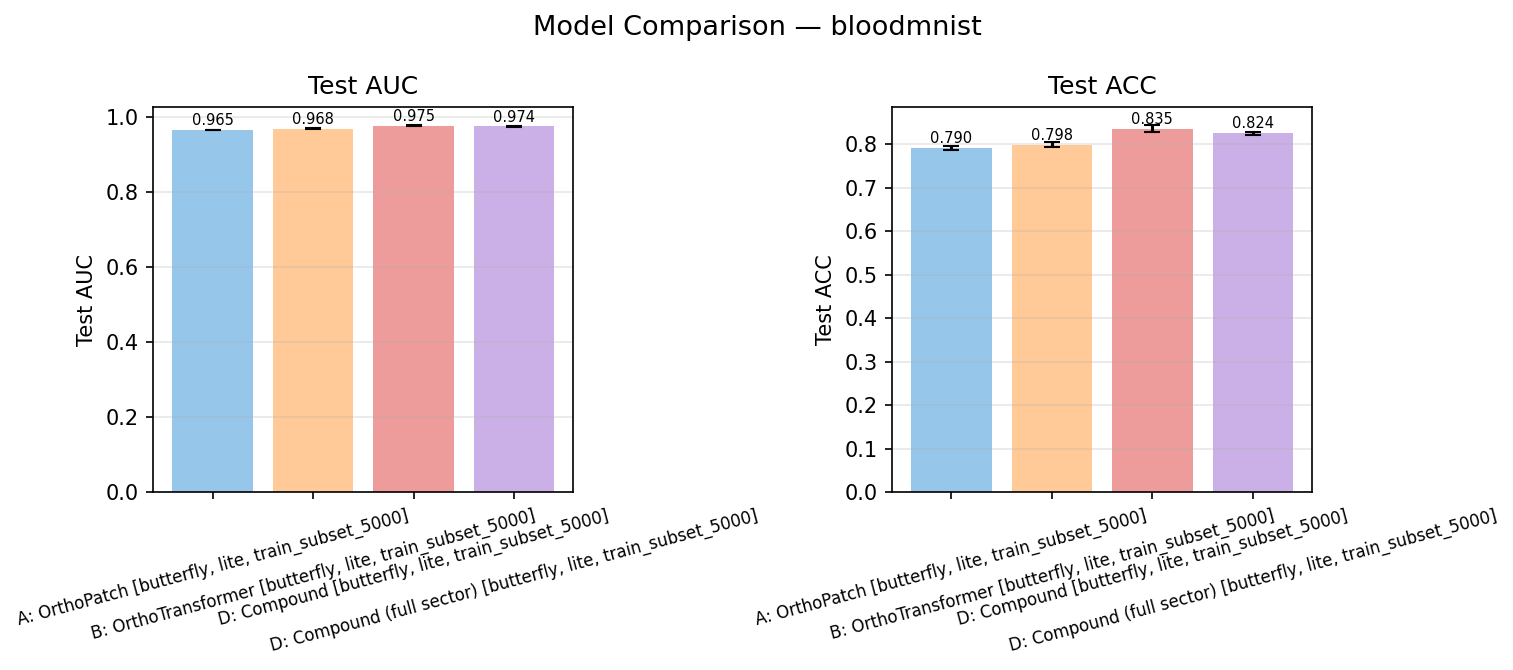
\includegraphics[width=\textwidth]{../../figures/butterfly/lite/comparison_bloodmnist.png}
\caption{BloodMNIST butterfly-lite comparison.}
\label{fig:bloodmnist}
\end{figure}

\begin{figure}[tbp]
\centering
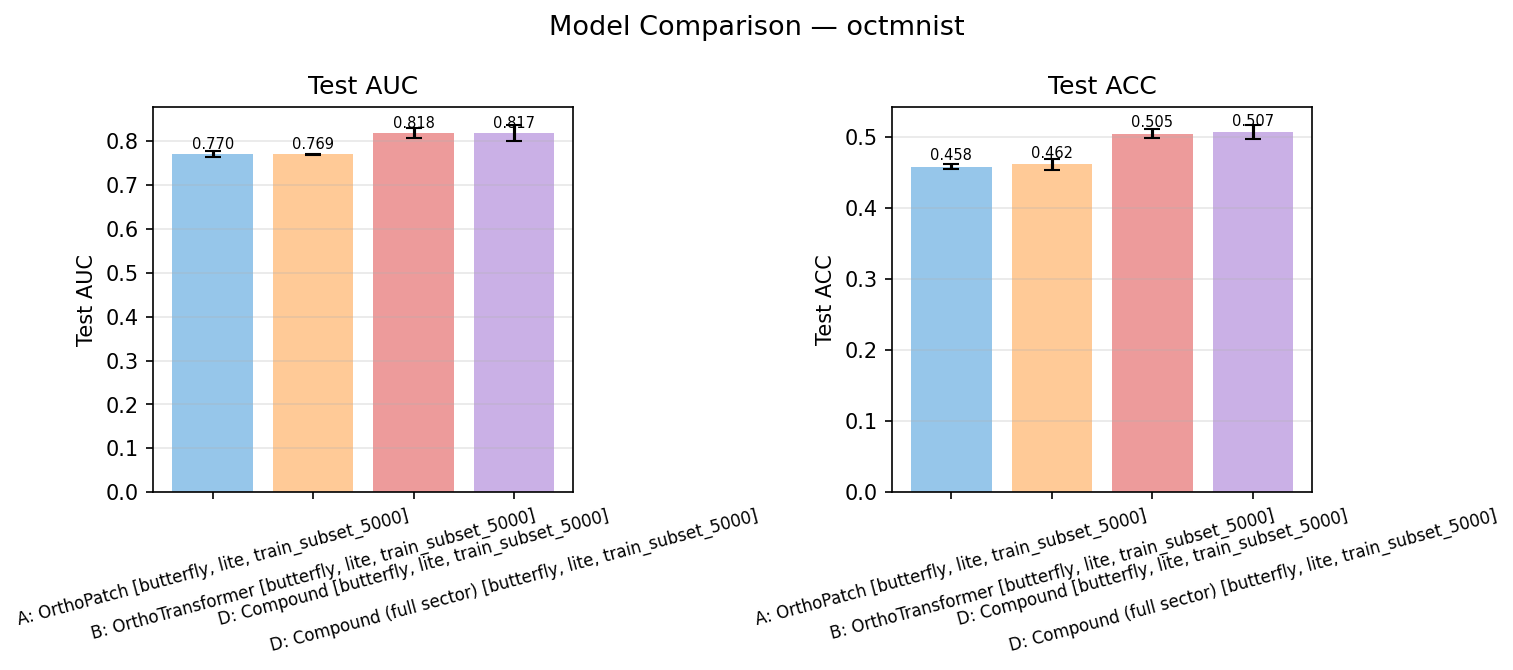
\includegraphics[width=\textwidth]{../../figures/butterfly/lite/comparison_octmnist.png}
\caption{OCTMNIST butterfly-lite comparison.}
\label{fig:octmnist}
\end{figure}

The overall pattern is now fairly clear. Under the 5000-example capped-data regime, the \texttt{D} family is strongest overall. Either \texttt{D} or \texttt{D\_full} achieves the best AUC on most datasets, and the same family often leads on ACC as well. At the same time, \texttt{A} remains surprisingly competitive and therefore remains the most attractive efficiency candidate. \texttt{B} is meaningful, but it is less consistently strong than the compound family. In that sense, the MedMNIST extension study reinforces rather than contradicts the paper's intuition that more structured quantum attention mechanisms are worth pursuing.

\section{Extensions Beyond the Paper}

The paper benchmark family ends at \texttt{D}, but the current repository already provides enough evidence to rank the extensions. The strongest extension is \texttt{D\_full}. It performs strongly on RetinaMNIST lite, it produces the best PathMNIST result in the capped-data study, and even when it does not clearly outperform \texttt{D}, it usually stays close enough to justify continued attention. If one extension deserves to be treated as a genuine follow-on research direction, it is \texttt{D\_full}.

The situation for \texttt{E} and \texttt{F} is different. \texttt{E} is interesting as a shared-circuit multi-sector hypothesis, but the empirical evidence in its favor is still weak. \texttt{F} is more conceptually compelling because it is a genuine three-photon extension and therefore points toward a broader higher-order compound family. However, it remains under-validated. The present ranking is therefore \texttt{D\_full} first, \texttt{F} second, and \texttt{E} third.

\section{Discussion Relative to the Paper's Main Claims}

The paper's qualitative narrative survives the current reproduction better than its exact numerical story. The repository clearly supports the claim that structured quantum models can be competitive with a classical transformer baseline. It also strongly supports the paper's parameter-efficiency argument. Finally, it supports the claim that the compound family is especially promising: both \texttt{D} and \texttt{D\_full} now look like the most scientifically fruitful line in the repository.

What the repository does not yet support is a literal reconstruction of every benchmark claim in the exact form reported in the paper. The repository has not completed a paper-style full-dataset MedMNIST sweep across all twelve datasets for the exact benchmark family. Model \texttt{B} remains weaker than the paper suggests. The baseline side is no longer provisional, but it remains a clear quantitative mismatch because \texttt{OrthoFNN} still trails the paper after the paper-faithful rerun. These caveats are real, and they matter if one wants to frame the result as a strict replication rather than as a scientifically credible qualitative reproduction.

\section{Conclusion}

The most accurate scientific conclusion is that the repository now supports a strong qualitative reproduction of \papertitle{}, but not yet an exact numerical reproduction of every reported benchmark value. That conclusion is justified because the main paper family is implemented and has been run, the training setup closely matches the paper, the strongest quantum models remain competitive with the classical baseline, and the quantum parameter-efficiency claim is strongly supported by the regenerated figures. The result is not a perfect reproduction because of the remaining \texttt{B} weakness, the completed but still underperforming paper-faithful \texttt{OrthoFNN} baseline, the unfinished tail of the MedMNIST plain-\texttt{D} capped-data sweep, and the unresolved architectural ambiguity around butterfly \texttt{D} and CLS-token usage.

The broader scientific message is also clear. The compound family is the most promising direction in the present codebase, \texttt{D\_full} is the extension with the strongest empirical case, and lite or capped-data regimes can preserve much of the useful behavior of the full models. In that respect, the repository has already progressed beyond a binary reproduction exercise and has become a meaningful platform for follow-on architectural study.

\section{Limitations and Future Work}

The first immediate priority is to finish the remaining plain-\texttt{D} OCTMNIST and TissueMNIST subset5000 runs so the capped-data MedMNIST study is fully clean. After that, the report can be rebuilt without the current completion caveat on those rows.

Beyond cleanup, the scientific priorities are already visible. \texttt{A}, \texttt{D}, and \texttt{D\_full} should remain the central models for further study. \texttt{D\_full} is the clearest extension worth pursuing aggressively. Large broad sweeps for \texttt{E} are lower priority, while broader work on \texttt{F} should wait until \texttt{D\_full} has been better exhausted as a research direction.

\end{document}
